\documentclass{udpreport}
%\headertext{Metodos Numéricos}
\title{Metodos Numéricos : Tarea 1}
\author{Thomas Muñoz , Diego Vilches , Javiera Araya , Ignacio Yanjari.}
\usepackage{amssymb}
\usepackage{amsmath}
\usepackage{graphicx}
\usepackage{float}
\usepackage{array}
\graphicspath{ {Imagenes/} }
\usepackage{listings}
\usepackage{color}

\definecolor{dkgreen}{rgb}{0,0.6,0}
\definecolor{gray}{rgb}{0.5,0.5,0.5}
\definecolor{mauve}{rgb}{0.58,0,0.82}

\lstset{frame=tb,
  language=MATLAB,
  aboveskip=3mm,
  belowskip=3mm,
  showstringspaces=false,
  columns=flexible,
  basicstyle={\small\ttfamily},
  numbers=none,
  numberstyle=\tiny\color{gray},
  keywordstyle=\color{blue},
  commentstyle=\color{dkgreen},
  stringstyle=\color{mauve},
  breaklines=true,
  breakatwhitespace=true,
  tabsize=4
}

\begin{document}
\maketitle
\tableofcontents
\listoffigures
\chapter{Introducción}

\chapter{Resolución de sistema de ecuaciones lineales} % rellenar con lo que corresponda
 \section{Programación}
 
 \section{Aplicación de los esquemas programados}
 \begin{enumerate}
 	\item
 		\begin{enumerate}
 			\item 	
 			\begin{figure}[H]
 				\centering
 				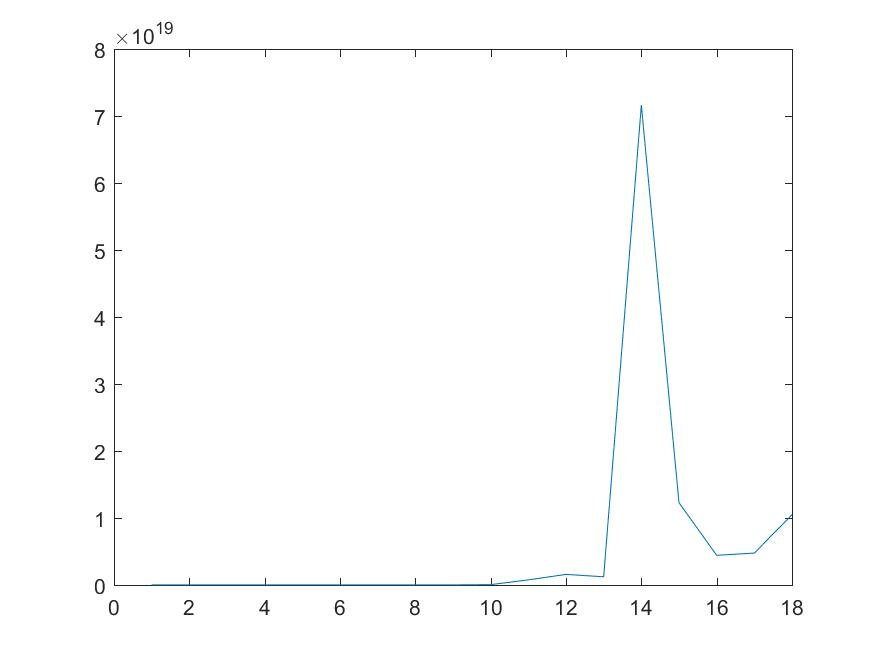
\includegraphics[width=9cm]{grafo1-a}
 				\caption{Gráfico del número de condición para una matriz de Hilbert de tamaño n}
 			\end{figure}
 			Se puede observar que entre más grande es el tamaño de la matriz de Hilbert, más grande es su número de condición. Este, al estar significativamente alejado del 1, implica que la matriz está mal condicionada.  %explica que significa que esté mal condicionada
 			\item 
 			\item \begin{figure}[H]
 				\centering
 				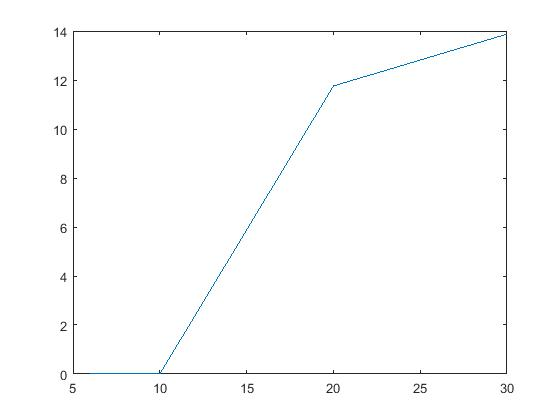
\includegraphics[width=9cm]{grafo1-rfe}
 				%\caption{}
 			\end{figure}
 		
 		
 		\end{enumerate}
	
 		
 \end{enumerate}
\newpage
\chapter{Algo 2}
    

     
 \newpage

    
    
\chapter{Conclusión}
      

\end{document}
